\Acrfull{nns} is a topic that attracted much active interest in the machine
learning research field as its exhaustive solutions require a lot of time and
resources to find the solution. It can find its applications as a fundamental
approach in multiple areas as recommendation systems, searching in multimedia
data, information retrieval, as well as in pattern recognition to name but a
few.

The problem of \Acrlong{nns} is formulated given a set of $n$ points of
dimension $d$ and a \gls{query} point $q$, it is concerned with finding the
point (or points) closest to this query point. In the figure
\ref{fig:nss_problem}, a basic example is presented on the left with 09 points
and a query point, the algorithm should return the point $s$ as the nearest
neighbor.
\begin{figure}[h]
    \centering
    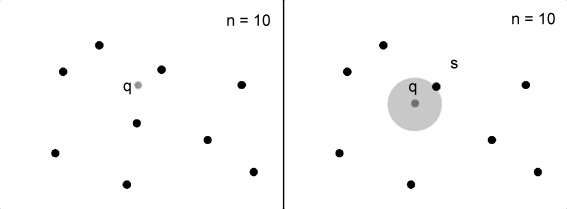
\includegraphics[width=\textwidth]{state_of_the_art/nss.jpg}
    \caption{Basic example of \Acrlong{nns}}
    \label{fig:nss_problem}
\end{figure}

The simplest solution, or the native solution is to compute the distance between
the query point and all the other points with a chosen metric. This solution
guarantees to return the exact nearest neighbor, but its computational
complexity is at the order of $O(nd)$ which will make it become more and more
complex with the explosive growth in the scale of datasets (when the number of points
and their dimension get bigger), that's what is called Curse of Dimensionality
problem where the accurate algorithms wouldn't meet the requirements to
guarantee the efficiency of the solution. Thus, the exact nearest neighbor
problem has been reformulated into (\Acrlong{ann}) where the focus is on
improving the efficiency of the solution with a tradeoff on the accuracy
\citep{fast_ann_hajebi_2011}.